\chapter{Transformadors de Pot\`{e}ncia}\index{transformadors de pot\`{e}ncia}

Es tracten en aquest cap\'{\i}tol els transformadors de pot\`{e}ncia
monof\`{a}sics i trif\`{a}sics des del punt de vista el\`{e}ctric, utilitzant els seus esquemes equivalents.

\section{Esquema equivalent i placa de caracter\'{\i}stiques}

\subsection{Esquema equivalent}\index{transformadors de pot\`{e}ncia!esquema equivalent}

Es presenta en primer lloc en la Figura \vref{pic:tr-pot-esquema-equiv} l'esquema el\`{e}ctric equivalent d'un transformador.
L'esquema \'{e}s v\`{a}lid tant per a un transformador monof\`{a}sic com per a un de trif\`{a}sic. En el cas d'un transformador trif\`{a}sic, l'esquema representa el circuit equivalent per fase, \'{e}s a dir l'esquema fase--neutre; els valors per fase s\'{o}n independents de que la connexi\'{o} dels debanats primari i secundari siguin en estrella, triangle o ziga-zaga.

\begin{figure}[htb]
\centering
    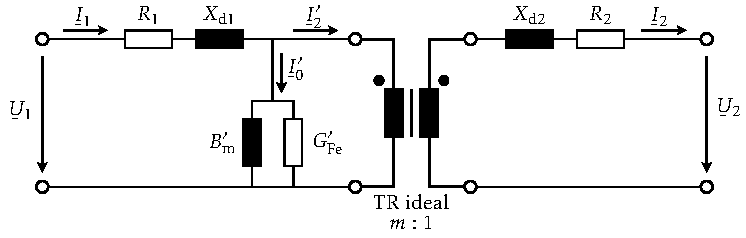
\includegraphics{Imatges/Cap-TrafosPot-Esq-Equiv.pdf}
\caption{Esquema equivalent d'un transformador}
\label{pic:tr-pot-esquema-equiv}
\end{figure}

En aquest esquema equivalent $R_1$ i $X\ped{d1}$ representen la resist\`{e}ncia i la react\`{a}ncia de dispersi\'{o} respectivament, del debanat primari, i de forma an\`{a}loga, $R_2$ i $X\ped{d2}$ representen la resist\`{e}ncia i la react\`{a}ncia de dispersi\'{o} respectivament, del debanat secundari; aquestes quatre magnituds es mesuren en ohm. Per la seva banda, $G\ped{Fe}'$ i $B\ped{m}'$ representen la conduct\`{a}ncia de p\`{e}rdues en el ferro i la suscept\`{a}ncia de magnetitzaci\'{o} respectivament, vistes des del primari; aquestes dues magnituds es mesuren en siemens.

Contr\`{a}riament al que passa amb les resist\`{e}ncies i react\`{a}ncies de dispersi\'{o} dels debanats, la conduct\`{a}ncia $G\ped{Fe}'$ i la suscept\`{a}ncia $B\ped{m}'$ no pertanyen a cap debanat, si no que s\'{o}n pr\`{o}pies del transformador; \'{e}s per aix\`{o} que es parla de valors vistos des del primari (com en la Figura \vref{pic:tr-pot-esquema-equiv}) o vistos des del secundari, representant-los en el costat corresponent.

La tensi\'{o} i corrent de primari s\'{o}n $\cmplx{U}_1$ i $\cmplx{I}_1$ respectivament, la tensi\'{o} i corrent de secundari s\'{o}n $\cmplx{U}_2$ i $\cmplx{I}_2$ respectivament, el corrent de secundari vist des del primari \'{e}s $\cmplx{I}_2'$, i el corrent de buit vist des del primari \'{e}s $\cmplx{I}_0'$.

Entre el primari i el secundari es co{\l.l}oca un transformador ideal (sense p\`{e}rdues) amb una relaci\'{o} de transformaci\'{o} $m$ igual a la del transformador real.

Els par\`{a}metres d'aquest esquema equivalent es poden agrupar en una imped\`{a}ncia de primari $\cmplx{Z}_1$, una imped\`{a}ncia de secundari $\cmplx{Z}_2$ i una  admit\`{a}ncia transversal vista des del primari: $\cmplx{Y}_0'$:
\begin{align}
    \cmplx{Z}_1 &= R_1 + \ju X\ped{d1} \\
    \cmplx{Z}_2 &= R_2 + \ju X\ped{d2}\\
    \cmplx{Y}_0' &= G\ped{Fe}'- \ju B\ped{m}'
\end{align}

Si es vol, la imped\`{a}ncia de secundari $\cmplx{Z}_2$ es pot passar al costat primari del transformador ideal, quedant aix\'{\i} un valor $\cmplx{Z}_2'$ referit al primari, de valor:
\begin{equation}
    \cmplx{Z}_2' = m^2 (R_2 + \ju X\ped{d2})
\end{equation}

Les equacions que lliguen les magnituds de la Figura \vref{pic:tr-pot-esquema-equiv} s\'{o}n:
\begin{align}
    \cmplx{U}_1  &=   \cmplx{Z}_1 \cmplx{I}_1 + \frac{\cmplx{I}_0'}{\cmplx{Y}_0'} \\
    \cmplx{U}_2  &= - \cmplx{Z}_2 \cmplx{I}_2 + \frac{\cmplx{I}_0'}{m \cmplx{Y}_0' }\\
    \cmplx{I}_1  &=   \cmplx{I}_2' + \cmplx{I}_0'\\
    \cmplx{I}_2' &=   \frac{\cmplx{I}_2}{m}
\end{align}

\subsection{Placa de caracter\'{\i}stiques}\index{transformadors de pot\`{e}ncia!placa de caracter\'{\i}stiques}

La  placa de caracter\'{\i}stiques d'un transformador recull els valors nominals  i els valors dels assajos
en buit i en curt circuit. El par\`{a}metres inclosos normalment s\'{o}n:
\begin{dinglist}{'167}
   \item Tensions nominals de primari i secundari,  $U\ped{N1}$ i $U\ped{N2}$: S\'{o}n les tensions que cal aplicar als debanats del transformador, per tal que funcioni correctament en r\`{e}gim permanent. Es poden admetre sobretensions del 5 \% en condicions de funcionament no permanent; la tensi\'{o} m\`{a}xima de l'a\"{\i}llament el\`{e}ctric determina la tensi\'{o} m\`{a}xima que pot suportar el transformador.
   \item Corrents nominals de primari i secundari,  $I\ped{N1}$ i $I\ped{N2}$: S\'{o}n els corrents m\`{a}xims que poden circular pels debanats del transformador en r\`{e}gim permanent. En condicions de funcionament no permanent s'admeten sobrec\`{a}rregues.
   \item Pot\`{e}ncia nominal, $S\ped{N}$: \'{E}s la pot\`{e}ncia aparent que s'obt\'{e} a partir de les tensions i corrents nominals de primari i secundari.
       \begin{equation}
        S\ped{N} = \begin{cases} U\ped{N1} I\ped{N1} = U\ped{N2} I\ped{N2}, & \text{transformador monof\`{a}sic} \\
        \sqrt{3} U\ped{N1} I\ped{N1} = \sqrt{3} U\ped{N2} I\ped{N2}, & \text{transformador trif\`{a}sic} \end{cases}
       \end{equation}
   \item Relaci\'{o} de transformaci\'{o}, $m$: \'{E}s la relaci\'{o} entre les tensions nominals de primari i secundari, i es calcula com la relaci\'{o} entre ambdues tensions, quan el primari est\`{a} connectat a la tensi\'{o} nominal i el secundari est\`{a} en buit. La relaci\'{o} de  transformaci\'{o} tamb\'{e} es pot calcular a partir del nombre d'espires del primari $N_1$ i del secundari $N_2$.\index{transformadors de pot\`{e}ncia!relaci\'{o} de transformaci\'{o}}
       \begin{equation}
        m = \frac{U\ped{N1}}{U\ped{N2}} =  \begin{cases}
        \dfrac{N_1}{N_2}, & \text{transformador monof\`{a}sic} \\[0.4cm]
        \dfrac{N_1}{N_2}, & \text{transformador trif\`{a}sic triangle--triangle} \\[0.4cm]
        \dfrac{\sqrt{3}N_1}{\sqrt{3}N_2} = \dfrac{N_1}{N_2}, & \text{transformador trif\`{a}sic estrella--estrella} \\[0.4cm]
        \dfrac{N_1}{\sqrt{3}N_2}, & \text{transformador trif\`{a}sic triangle--estrella} \\[0.4cm]
        \dfrac{\sqrt{3}N_1}{N_2}, & \text{transformador trif\`{a}sic estrella--triangle} \\[0.4cm]
        \dfrac{N_1}{\frac{3}{2}N_2} = \dfrac{2 N_1}{3 N_2}, & \text{transformador trif\`{a}sic triangle--ziga-zaga} \\[0.4cm]
        \dfrac{\sqrt{3}N_1}{\frac{3}{2}N_2} = \dfrac{2 N_1}{\sqrt{3} N_2}, & \text{transformador trif\`{a}sic estrella--ziga-zaga}
         \end{cases}
       \end{equation}
   \item Freq\"{u}\`{e}ncia nominal, $f\ped{N}$: Freq\"{u}\`{e}ncia a la qual corresponen la resta de valors nominals.
   \item Connexi\'{o} trif\`{a}sica: En el cas de transformadors trif\`{a}sics, s'especifica la connexi\'{o} (estrella, triangle o ziga-zaga) de cadascun dels dos debanats, aix\'{\i} com el desfase entre les tensions de primari i secundari (vegeu la secci\'{o}\vref{sec:connex-index-horari}).
   \item Dades de l'assaig en buit, $i\ped{o}$ i $W\ped{o}$ i de l'assaig en curt circuit, $\varepsilon\ped{cc}$ i $W\ped{cc}$: Els valors de les pot\`{e}ncies $W\ped{o}$ i $W\ped{cc}$ es donen
usualment en watt, mentre que els valors dels par\`{a}metres $i\ped{o}$
i $\varepsilon\ped{cc}$ es donen en p.u. o en tant per cent; a partir d'aquest valors es pot calcular els valors dels par\`{a}metres de l'esquema equivalent del transformador  (vegeu la secci\'{o} \vref{sec:determ-param-trafo}).

\end{dinglist}

Un transformador pot funcionar en unes condicions diferents a les nominals, com per exemple:
\begin{dinglist}{'167}
   \item Pot treballar a tensions nominals per\`{o} subministrant una pot\`{e}ncia inferior a la nominal; aquest \'{e}s el cas de funcionament m\'{e}s com\'{u}.
   \item Pot treballar a tensions inferior a la nominal, per\`{o} donat que el corrent no ha de superar el seu valor nominal, la pot\`{e}ncia subministrada haur\`{a} de ser menor que la nominal.
   \item Pot treballar a altres freq\"{u}\`{e}ncies diferents de la nominal; per a freq\"{u}\`{e}ncies superiors cal tenir en compte que les p\`{e}rdues seran tamb\'{e} superiors, i per tant la pot\`{e}ncia subministrada haur\`{a} de ser menor que la nominal.
\end{dinglist}

\section{Esquemes equivalents redu\"{\i}ts}

Quan es volen fer c\`{a}lculs en circuits el\`{e}ctrics amb transformadors, l'esquema equivalent d'un transformador de la Figura  \vref{pic:tr-pot-esquema-equiv}, presenta l'inconvenient d'incorporar un transformador ideal. \'{E}s per aix\`{o} que interessa m\'{e}s utilitzar esquemes redu\"{\i}ts on aquest transformador ideal desaparegui.

El proc\'{e}s utilitzat \'{e}s b\`{a}sicament el que ja s'ha descrit en la secci\'{o} \vref{sec:seccio_pu}. S'escull una pot\`{e}ncia base $S\ped{B}$, una tensi\'{o} base pel primari $U\ped{B1}$, i una tensi\'{o} base pel secundari $U\ped{B2}$; els valors base de primari i secundari dels corrents $I\ped{B1}$ i $I\ped{B2}$, de les imped\`{a}ncies $Z\ped{B1}$ i $Z\ped{B2}$ i de les admit\`{a}ncies $Y\ped{B1}$ i $Y\ped{B2}$, es calculen a partir de $S\ped{B}$, $U\ped{B1}$ i $U\ped{B2}$.

La condici\'{o} que han de satisfer $U\ped{B1}$ i $U\ped{B2}$ per tal que el transformador ideal de l'esquema redu\"{\i}t desaparegui, \'{e}s que donin lloc a una relaci\'{o} de transformaci\'{o} del transformador ideal redu\"{\i}t $m\ped{r}$ igual a  1:
\begin{equation}\label{eq:mr}
    m\ped{r} = 1 \quad \Rightarrow \quad \frac{U\ped{B1}}{U\ped{B2}} = \frac{U\ped{N1}}{U\ped{N2}} = m
\end{equation}

 Amb aquesta condici\'{o}, l'esquema de la Figura \vref{pic:tr-pot-esquema-equiv} es converteix en l'esquema de la Figura
\vref{pic:tr-pot-esquema-equiv-reduit-T}, anomenat usualment esquema redu\"{\i}t en {"<}T{">}.\index{transformadors de pot\`{e}ncia!esquema redu\"{\i}t en \guillemotleft T\guillemotright}

\begin{figure}[htb]
\centering
    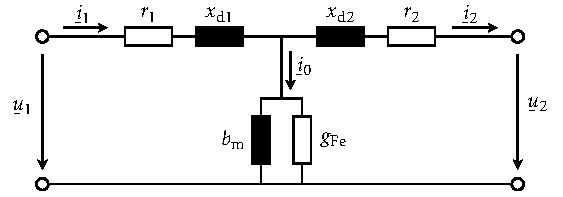
\includegraphics{Imatges/Cap-TrafosPot-Esq-Equiv-Reduit-T.pdf}
\caption{Esquema redu\"{\i}t en {"<}T{">} d'un transformador}
\label{pic:tr-pot-esquema-equiv-reduit-T}
\end{figure}

Els valors dels par\`{a}metres de l'esquema equivalent redu\"{\i}t en {"<}T{">}, s'obtenen dividint els valors dels par\`{a}metres reals pels valors base corresponents:
\begin{align}
    r\ped{1} &=\frac{R\ped{1}}{Z\ped{B1}} &   x\ped{d1} &=\frac{X\ped{d1}}{Z\ped{B1}} \\[1ex]
    r\ped{2} &=\frac{R\ped{2}}{Z\ped{B2}} &   x\ped{d2} &=\frac{X\ped{d2}}{Z\ped{B2}} \\[1ex]
    b\ped{m} &=\frac{B\ped{m}'}{Y\ped{B1}}  &   g\ped{Fe} &=\frac{G\ped{Fe}'}{Y\ped{B1}} \\[1ex]
    \cmplx{u}_1 &=\frac{\cmplx{U}_1}{U\ped{B1}} &   \cmplx{i}_1 &=\frac{\cmplx{I}_1}{I\ped{B1}} \\[1ex]
    \cmplx{u}_2 &=\frac{\cmplx{U}_2}{U\ped{B2}} &   \cmplx{i}_2 &=\frac{\cmplx{I}_2}{I\ped{B2}} \\[1ex]
    \cmplx{i}_0 &=\frac{\cmplx{I}_0'}{I\ped{B1}} &   m\ped{r} &=1
\end{align}

Un cop es tenen els valor redu\"{\i}ts es treballa amb aquest esquema con si es tract\'{e}s d'un circuit monof\`{a}sic fase--neutre, independentment de si el transformador real original era monof\`{a}sic o trif\`{a}sic.

En la pr\`{a}ctica, degut al petit error com\`{e}s i a que no sempre es disposa per separat de les imped\`{a}ncies prim\`{a}ries i secund\`{a}ries,  s'ajunten aquests valors en una resist\`{e}ncia \'{u}nica $r= r\ped{1}+r\ped{2}$  i una imped\`{a}ncia \'{u}nica $x= x\ped{d1}+x\ped{d2}$ ; per convenci\'{o} $r$ i $x$ se situen en el costat d'alta tensi\'{o}. Per tant, depenent de que el costat d'alta tensi\'{o} es trobi en el primari o en el secundari,  tenim els esquemes redu\"{\i}ts de la Figura \vref{pic:tr-pot-esquema-equiv-reduit-L}, anomenats usualment esquemes redu\"{\i}ts en {"<}L{">}. El valor $\cmplx{z}\ped{cc} = r + \ju x$ es coneix com a imped\`{a}ncia de curt circuit. \index{transformadors de pot\`{e}ncia!esquemes redu\"{\i}ts en \guillemotleft L\guillemotright}
\begin{figure}[htb]
\centering
    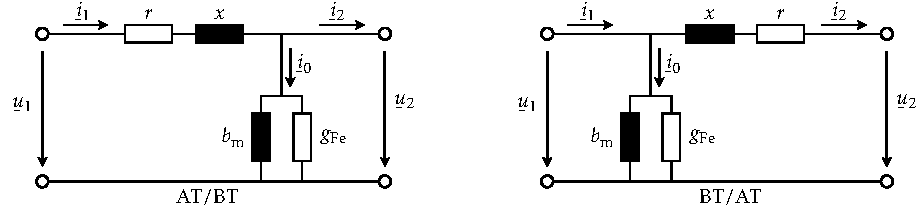
\includegraphics{Imatges/Cap-TrafosPot-Esq-Equiv-Reduit-L.pdf}
\caption{Esquemes redu\"{\i}ts en {"<}L{">} d'un transformador}
\label{pic:tr-pot-esquema-equiv-reduit-L}
\end{figure}

Finalment, quan el transformador treballa en c\`{a}rrega, \'{e}s a dir, \'{e}s lluny de treballar en buit i es compleix $|\cmplx{i}_2| \gg |\cmplx{i}_0|$, es pot eliminar l'admit\`{a}ncia transversal en els esquemes equivalents redu\"{\i}ts en {"<}T{">} o en {"<}L{">}, ja que l'error com\`{e}s \'{e}s molt petit.

En la  Taula \vref{taula:valors-base} es relacionen els valors base dels tres tipus d'esquemes equivalents redu\"{\i}ts m\'{e}s utilitzats: l'esquema en p.u., l'esquema redu\"{\i}t al primari i l'esquema redu\"{\i}t al secundari.\index{transformadors de pot\`{e}ncia!valors base}

\begin{longtable}{ccccccc}
\caption{\label{taula:valors-base}Valors base per a diferents tipus d'esquemes redu\"{\i}ts} \\
\toprule[1pt]
    \renewcommand*{\multirowsetup}{\centering}
    \multirow{2}{12mm}{\rule{0mm}{4mm}Valor\\{Base}}  &    \multicolumn{3}{c}{Transformador monof\`{a}sic} &   \multicolumn{3}{c}{Transformador trif\`{a}sic}         \\
    \cmidrule(rl){2-4} \cmidrule(rl){5-7}
      &    \multicolumn{1}{c}{en p.u.}  & \multicolumn{1}{c}{redu\"{\i}t al 1ari}  & \multicolumn{1}{c}{redu\"{\i}t al 2ari}
           &    \multicolumn{1}{c}{en p.u.} &   \multicolumn{1}{c}{redu\"{\i}t al 1ari}  & \multicolumn{1}{c}{redu\"{\i}t al 2ari} \\
\midrule \endfirsthead
\caption[]{Valors base per a diferents tipus d'esquemes redu\"{\i}ts (\emph{ve de la p\`{a}gina anterior})} \\
\toprule[1pt]
    \renewcommand*{\multirowsetup}{\centering}
    \multirow{2}{12mm}{\rule{0mm}{4mm}Valor\\{Base}}  &    \multicolumn{3}{c}{Transformador monof\`{a}sic} &   \multicolumn{3}{c}{Transformador trif\`{a}sic}         \\
    \cmidrule(rl){2-4} \cmidrule(rl){5-7}
      &    \multicolumn{1}{c}{en p.u.}  & \multicolumn{1}{c}{redu\"{\i}t al 1ari}  & \multicolumn{1}{c}{redu\"{\i}t al 2ari}
           &    \multicolumn{1}{c}{en p.u.} &   \multicolumn{1}{c}{redu\"{\i}t al 1ari}  & \multicolumn{1}{c}{redu\"{\i}t al 2ari} \\
\midrule \endhead
\midrule
\multicolumn{7}{r}{(\emph{continua a la p\`{a}gina seg\"{u}ent})}
\endfoot
\endlastfoot
$S\ped{B}$ [VA] &      $S\ped{N}$ &   1 &     1  &      $S\ped{N}$  &  3 &   3 \\[0.4cm]
$U\ped{B1}$ [V] & $U\ped{N1}$ & 1 & $m$ & $U\ped{N1}$ & $\sqrt{3}$  & $\sqrt{3} m$\\[0.4cm]
$U\ped{B2}$ [V] & $U\ped{N2}$ & $\dfrac{1}{m}$ & 1 & $U\ped{N2}$ & $\dfrac{\sqrt{3}}{m}$ & $\sqrt{3}$ \\[0.4cm]
$I\ped{B1}$ [A] & $\dfrac{S\ped{N}}{U\ped{N1}}$ & 1 & $\dfrac{1}{m}$ & $\dfrac{S\ped{N}}{\sqrt{3}U\ped{N1}}$ & 1  & $\dfrac{1}{m}$\\[0.4cm]
$I\ped{B2}$ [A] & $\dfrac{S\ped{N}}{U\ped{N2}}$  & $m$ & 1 & $\dfrac{S\ped{N}}{\sqrt{3}U\ped{N2}}$   & $m$ & 1\\[0.4cm]
$Z\ped{B1}$ [$\ohm$]& $\dfrac{U\ped{N1}^2}{S\ped{N}}$ & 1 & $m^2$ & $\dfrac{U\ped{N1}^2}{S\ped{N}}$ & 1 & $m^2$\\[0.4cm]
$Z\ped{B2}$ [$\ohm$]& $\dfrac{U\ped{N2}^2}{S\ped{N}}$  & $\dfrac{1}{m^2}$ & 1& $\dfrac{U\ped{N2}^2}{S\ped{N}}$  & $\dfrac{1}{m^2}$ & 1\\[0.4cm]
$Y\ped{B1}$ [S]& $\dfrac{S\ped{N}}{U\ped{N1}^2}$ & 1 & $\dfrac{1}{m^2}$ & $\dfrac{S\ped{N}}{U\ped{N1}^2}$ & 1 & $\dfrac{1}{m^2}$ \\[0.4cm]
$Y\ped{B2}$ [S]& $\dfrac{S\ped{N}}{U\ped{N2}^2}$  & $m^2$ & 1 & $\dfrac{S\ped{N}}{U\ped{N2}^2}$ &$m^2$ &  1\\[0.4cm]
\bottomrule[1pt]
\end{longtable}

Com \'{e}s usual en el cas de circuits trif\`{a}sics, les pot\`{e}ncies s\'{o}n  pot\`{e}ncies trif\`{a}siques,  les tensions s\'{o}n  tensions fase--fase i l'esquema equivalent redu\"{\i}t \'{e}s un esquema equivalent fase--neutre.

Quan hi ha m\'{e}s d'un transformador en un circuit s'utilitza normalment l'esquema redu\"{\i}t en p.u., escollint una pot\`{e}ncia base \'{u}nica, i tantes tensions base con nivells de tensi\'{o}  originin els transformadors; cadascuna de les parelles de tensions base consecutives han de complir la relaci\'{o} de l'equaci\'{o} \eqref{eq:mr}. En la la secci\'{o} \vref{sec:canvi-base}) es pot veure un exemple amb dos transformadors.

\section{Circuit equivalent Th\'{e}venin vist des del secundari}\label{sec:trafo-thevenin}\index{transformadors de pot\`{e}ncia!circuit equivalent Th\'{e}venin}

El que s'explica a continuaci\'{o} \'{e}s v\`{a}lid per a transformadors
monof\`{a}sics i trif\`{a}sics, ja que s'utilitzar\`{a} l'esquema equivalent del
transformador en {"<}T{">}, expressant tots els seus valors en p.u.

En la Figura \vref{pic:esq_equiv_thev_trafo_sec}  es representa a
l'esquerra, un transformador alimentat des del primari per una font
de tensi\'{o} $\cmplx{u}\ped{G}$, la qual t\'{e} una imped\`{a}ncia s\`{e}rie
$\cmplx{z}\ped{G}$, i a  la dreta, el seu circuit equivalent
Th\'{e}venin.

\begin{figure}[htb]
\centering
    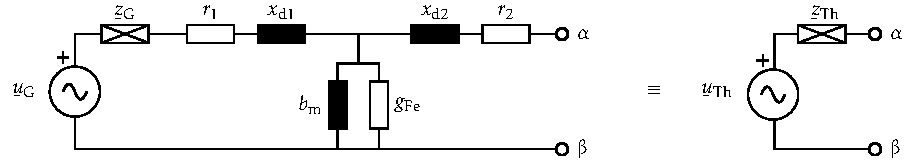
\includegraphics{Imatges/Cap-TrafosPot-Esq-Equiv-Thevenin.pdf}
\caption{Circuit equivalen Th\'{e}venin d'un transformador vist des del
secundari} \label{pic:esq_equiv_thev_trafo_sec}
\end{figure}

La tensi\'{o} i imped\`{a}ncia Th\'{e}venin v\'{e}nen definides per les equacions
seg\"{u}ents:
\begin{align}
    \cmplx{u}\ped{Th} &= \frac{\cmplx{u}\ped{G}}{\cmplx{z}\ped{G} + r_1 + \ju
    x\ped{d1} + \dfrac{1}{g\ped{Fe}-\ju b\ped{m}}} \;\frac{1}{g\ped{Fe}-\ju
    b\ped{m}} \label{eq:trafo_uth}\\[1ex]
    \cmplx{z}\ped{Th} &= r_2 + \ju x\ped{d2} + \frac{1}{\dfrac{1}{\cmplx{z}\ped{G} + r_1 +
    \ju x\ped{d1}} + g\ped{Fe}-\ju b\ped{m}}\label{eq:trafo_zth}
\end{align}

Tal com s'ha explicat en l'apartat \vref{sec:T_N}, la tensi\'{o}
$\cmplx{u}\ped{Th}$ \'{e}s igual a la tensi\'{o} en buit entre $\alphaup$ i
$\betaup$, i la imped\`{a}ncia $\cmplx{z}\ped{Th}$ \'{e}s igual la imped\`{a}ncia
que existeix entre $\alphaup$ i $\betaup$ quan es curtcircuita la font
de tensi\'{o} $\cmplx{u}\ped{G}$.

Normalment no es coneixen $r_1$, $r_2$, $x\ped{d1}$ i $x\ped{d2}$ per separat, i
en canvi, s\'{\i} que es coneixen $r=r_1+r_2$ i $x=x\ped{d1}+x\ped{d2}$; en aquest
cas s'obtenen dues equacions aproximades, a partir de les equacions
anteriors, substituint $r_1$ i $x\ped{d1}$ per $r$ i $x$ respectivament en
les equacions de $\cmplx{u}\ped{Th}$ i $\cmplx{z}\ped{Th}$, i
menyspreant addicionalment el terme $r_2 + \ju x\ped{d2}$ en l'equaci\'{o}
de $\cmplx{z}\ped{Th}$. Amb aquestes consideracions tenim:
\begin{align}
    \cmplx{u}\ped{Th} &\approx \frac{\cmplx{u}\ped{G}}{\cmplx{z}\ped{G} + r + \ju
    x + \dfrac{1}{g\ped{Fe}-\ju b\ped{m}}} \;\frac{1}{g\ped{Fe}-\ju
    b\ped{m}} \label{eq:trafo_uth_aprx}\\[1ex]
    \cmplx{z}\ped{Th} &\approx \frac{1}{\dfrac{1}{\cmplx{z}\ped{G} + r +
    \ju x} + g\ped{Fe}-\ju b\ped{m}}\label{eq:trafo_zth_aprx}
\end{align}

A partir de les equacions \eqref{eq:trafo_uth} i
\eqref{eq:trafo_zth}, o de les equacions \eqref{eq:trafo_uth_aprx} i
\eqref{eq:trafo_zth_aprx}, si es vol treballar amb els valors
redu\"{\i}ts al secundari $\cmplx{U}\ped{Th}^{''}$ i
$\cmplx{Z}\ped{Th}^{''}$, nom\'{e}s cal multiplicar els valors en p.u.
que s'obtenen amb aquestes equacions, per les tensions i imped\`{a}ncies
base del secundari $U\ped{B2}$ i $Z\ped{B2}$ respectivament:
\begin{align}
    \cmplx{U}\ped{Th}^{''} &= \cmplx{u}\ped{Th} \, U\ped{B2} \\[1ex]
    \cmplx{Z}\ped{Th}^{''} &= \cmplx{z}\ped{Th} \, Z\ped{B2}
\end{align}


\section{Rendiment, caiguda de tensi\'{o} i regulaci\'{o} de voltatge}

\subsection{Rendiment}\index{transformadors de pot\`{e}ncia!rendiment}

El rendiment $\eta$ d'un transformador es calcula tenint en compte la pot\`{e}ncia activa subministrada en el secundari $p_2$ i les p\`{e}rdues de pot\`{e}ncia activa en el coure dels debanats $p\ped{Cu}$ i en el ferro del circuit magn\`{e}tic $p\ped{Fe}$:
\begin{equation}
    \eta = \frac{p_2}{p_2 + p\ped{Cu} + p\ped{Fe}}
\end{equation}

La pot\`{e}ncia $p_2$ ve determinada per la c\`{a}rrega connectada en el secundari del transformador, i utilitzant els esquemes equivalents redu\"{\i}ts es pot calcular com:
\begin{equation}
    p_2 = \Re(\cmplx{u}_2 \,\cmplx{i}_2^*)
\end{equation}

Les p\`{e}rdues de pot\`{e}ncies  en el coure i en el ferro es calculen, utilitzant els esquemes equivalents redu\"{\i}ts en {"<}L{">}, a partir de les expressions seg\"{u}ents:

\begin{equation}
\begin{array}{c}\text{Transformador}\\
\text{AT/BT}
\end{array} \left\{
\begin{array}{l}
   p\ped{Cu} = r |\cmplx{i}_1|^2 \\[2.7ex]
   p\ped{Fe} = g\ped{Fe} |\cmplx{u}_2|^2
\end{array}
\right. \qquad\qquad
\begin{array}{c}\text{Transformador}\\
\text{BT/AT}
\end{array} \left\{
\begin{array}{l}
   p\ped{Cu} = r |\cmplx{i}_2|^2 \\[2.5ex]
   p\ped{Fe} = g\ped{Fe} |\cmplx{u}_1|^2
\end{array}
\right.
\end{equation}

\subsection{Caiguda de tensi\'{o} i regulaci\'{o} de voltatge}\index{transformadors de pot\`{e}ncia!caiguda de tensi\'{o}}\index{transformadors de pot\`{e}ncia!regulaci\'{o} de voltatge}

La caiguda de tensi\'{o} d'un transformador $\Delta u$ es defineix con la difer\`{e}ncia entre la tensi\'{o} secund\`{a}ria quan el transformador est\`{a} en buit i aquesta mateixa tensi\'{o} quan el transformador treballa en c\`{a}rrega.

Observant els esquemes equivalents redu\"{\i}ts, es veu que quan el transformador treballa en buit tenim $\cmplx{i}_2=0$, i donat que la imped\`{a}ncia transversal \'{e}s molt m\'{e}s gran que la longitudinal, la tensi\'{o} en buit del secundari \'{e}s pr\`{a}cticament igual a la prim\`{a}ria. Per tant, la caiguda de tensi\'{o} \'{e}s:
\begin{equation}
    \Delta u = |\cmplx{u}_1| - |\cmplx{u}_2|
\end{equation}

Normalment aquest valor \'{e}s positiu, per\`{o} quan la carrega connectada al secundari es fortament capacitiva, podem tenir  $|\cmplx{u}_2| > |\cmplx{u}_1|$ i per tant una caiguda de tensi\'{o} negativa; aix\`{o} es coneix com a efecte Ferranti.

La regulaci\'{o} de voltatge RV no \'{e}s m\'{e}s que la caiguda de tensi\'{o} respecte la tensi\'{o} del secundari:
\begin{equation}
    RV = \frac{|\cmplx{u}_1| - |\cmplx{u}_2|}{|\cmplx{u}_2|}
\end{equation}

\section{Determinaci\'{o} dels par\`{a}metres el\`{e}ctrics}\label{sec:determ-param-trafo}\index{transformadors de pot\`{e}ncia!determinaci\'{o} de par\`{a}metres}

Els transformadors se sotmeten b\`{a}sicament a dos assajos, assaig en
buit i assaig en curt circuit, per tal de determinar els par\`{a}metres
del seus circuits el\`{e}ctrics equivalents.

Mitjan\c{c}ant l'assaig en buit es determinen els par\`{a}metres
transversals del circuit equivalent, i mitjan\c{c}ant l'assaig en curt
circuit es determinen els seus par\`{a}metres longitudinals.

Per realitzar aquest assajos, cal con\`{e}ixer pr\`{e}viament els par\`{a}metres
b\`{a}sics del transformador: les tensions nominals de primari i de
secundari $U\ped{N1}$ i $U\ped{N2}$, i la pot\`{e}ncia nominal
$S\ped{N}$; com \'{e}s habitual, en el cas dels transformadors
trif\`{a}sics, les tensions nominals s\'{o}n les tensions fase--fase, i la
pot\`{e}ncia nominal \'{e}s la pot\`{e}ncia trif\`{a}sica.

Els corrents nominals s'obtenen a partir de les tensions i pot\`{e}ncia
nominals:
\begin{equation}
\begin{array}{c}\text{Transformador}\\
\text{Monof\`{a}sic}
\end{array} \left\{
\begin{array}{l}
   I\ped{N1} = \dfrac{S\ped{N}}{U\ped{N1}} \\[2.7ex]
   I\ped{N2} = \dfrac{S\ped{N}}{U\ped{N2}}
\end{array}
\right. \qquad\qquad
\begin{array}{c}\text{Transformador}\\
\text{Trif\`{a}sic}
\end{array} \left\{
\begin{array}{l}
   I\ped{N1} = \dfrac{S\ped{N}}{\sqrt{3}U\ped{N1}} \\[2.5ex]
   I\ped{N2} = \dfrac{S\ped{N}}{\sqrt{3}U\ped{N2}}
\end{array}
\right.
\end{equation}

En les explicacions que v\'{e}nen a continuaci\'{o}, se suposa que el
primari \'{e}s el costat d'alta tensi\'{o}, i que el secundari \'{e}s el costat
de baixa tensi\'{o}. Amb aix\`{o}, no es perd la generalitat de
l'explicaci\'{o}, ja que si la configuraci\'{o} real es la contr\`{a}ria de la
adoptada aqu\'{\i}, \'{u}nicament caldr\`{a} intercanviar els sub\'{\i}ndexs 1 i 2, en
les equacions que s'exposaran tot seguit.

\subsection{Assaig en buit}\index{transformadors de pot\`{e}ncia!assaig en buit}

La manera m\'{e}s usual de fer l'assaig en buit, \'{e}s alimentar el costat
de baixa tensi\'{o} del transformador a  la seva tensi\'{o} nominal, tot
deixant el costat d'alta tensi\'{o} en circuit obert. Tamb\'{e} \'{e}s possible,
no obstant, alimentar pel costat d'alta tensi\'{o} i deixar en circuit
obert el costat de baixa tensi\'{o}; aix\'{\i} mateix, tampoc no \'{e}s necessari
alimentar a tensi\'{o} nominal, n'hi ha prou amb un valor proper.

En la Figura \vref{pic:assaig_buit_mono} es pot veure com ha de
connectar-se un transformador monof\`{a}sic, per tal de realitzar el seu
assaig en buit.

\begin{figure}[htb]
\centering
    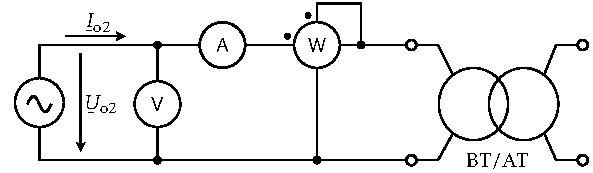
\includegraphics{Imatges/Cap-TrafosPot-Assaig-Buit-Monofasic.pdf}
\caption{Assaig en buit d'un transformador monof\`{a}sic}
\label{pic:assaig_buit_mono}
\end{figure}

A partir del diversos aparells de mesura, obtenim els valors de la
tensi\'{o} d'alimentaci\'{o} $U\ped{o2}$, del corrent que circula
$I\ped{o2}$, i de la pot\`{e}ncia consumida $W\ped{o}$, segons:
\begin{equation}
    U\ped{o2}\equiv|\cmplx{U}\ped{o2}|=\textsf{V} \qquad
    I\ped{o2}\equiv|\cmplx{I}\ped{o2}|=\textsf{A}
    \qquad W\ped{o}=\textsf{W}
\end{equation}

En la Figura \vref{pic:assaig_buit_trif} es pot veure com ha de
connectar-se un transformador trif\`{a}sic, per tal de realitzar el seu
assaig en buit.

\begin{figure}[h]
\centering
    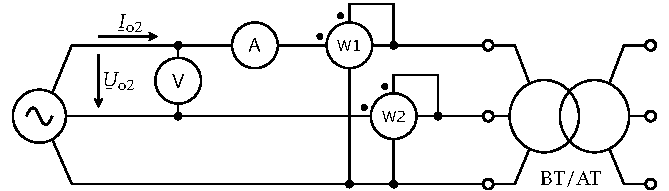
\includegraphics{Imatges/Cap-TrafosPot-Assaig-Buit-Trifasic.pdf}
\caption{Assaig en buit d'un transformador trif\`{a}sic}
\label{pic:assaig_buit_trif}
\end{figure}


A partir del diversos aparells de mesura, obtenim els valors de la
tensi\'{o} trif\`{a}sica d'alimentaci\'{o} $U\ped{o2}$, del corrent que circula
$I\ped{o2}$, i de la pot\`{e}ncia consumida $W\ped{o}$, segons:
\begin{equation}
    U\ped{o2}\equiv|\cmplx{U}\ped{o2}|=\textsf{V} \qquad
    I\ped{o2}\equiv|\cmplx{I}\ped{o2}|=\textsf{A} \qquad
    W\ped{o}=\textsf{W1}+\textsf{W2}
\end{equation}

\subsection{Assaig en curt circuit}\index{transformadors de pot\`{e}ncia!assaig en curt circuit}

La manera m\'{e}s usual de fer l'assaig en curt circuit, \'{e}s
curtcircuitar el costat de baixa tensi\'{o} del transformador, i
alimentar el costat d'alta tensi\'{o} a  una tensi\'{o} tal, que el corrent
que circuli sigui igual al nominal. Tamb\'{e} \'{e}s possible, no obstant,
alimentar pel costat de baixa tensi\'{o} i curtcircuitar el costat
d'alta tensi\'{o}; aix\'{\i} mateix, tampoc no \'{e}s necessari que el corrent
que circuli sigui el nominal, n'hi ha prou amb un valor proper.

En la Figura \vref{pic:assaig_cc_mono} es pot veure com ha de
connectar-se un transformador monof\`{a}sic, per tal de realitzar el seu
assaig en curt circuit.

\begin{figure}[htb]
\centering
    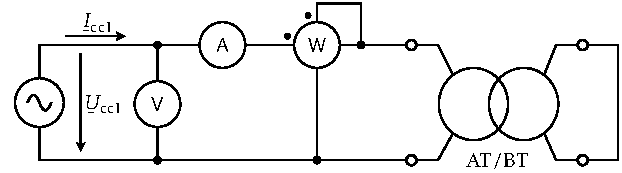
\includegraphics{Imatges/Cap-TrafosPot-Assaig-CC-Monofasic.pdf}
\caption{Assaig en curt circuit d'un transformador monof\`{a}sic}
\label{pic:assaig_cc_mono} \
\end{figure}

A partir del diversos aparells de mesura, obtenim els valors de la
tensi\'{o} d'alimentaci\'{o} $U\ped{cc1}$, del corrent que circula
$I\ped{cc1}$, i de la pot\`{e}ncia consumida $W\ped{cc}$, segons:
\begin{equation}
    U\ped{cc1}\equiv|\cmplx{U}\ped{cc1}|=\textsf{V} \qquad
    I\ped{cc1}\equiv|\cmplx{I}\ped{cc1}|=\textsf{A}
     \qquad W\ped{cc}=\textsf{W}
\end{equation}

En la Figura \vref{pic:assaig_cc_trif} es pot veure com ha de
connectar-se un transformador trif\`{a}sic, per tal de realitzar el seu
assaig en curt circuit.

\begin{figure}[htb]
\centering
    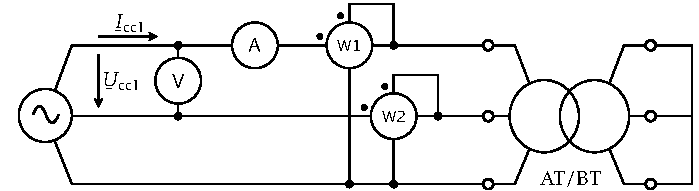
\includegraphics{Imatges/Cap-TrafosPot-Assaig-CC-Trifasic.pdf}
\caption{Assaig en curt circuit d'un transformador trif\`{a}sic}
\label{pic:assaig_cc_trif}
\end{figure}


A partir del diversos aparells de mesura, obtenim els valors de la
tensi\'{o} trif\`{a}sica d'alimentaci\'{o} $U\ped{cc1}$, del corrent que circula
$I\ped{cc1}$, i de la pot\`{e}ncia consumida $W\ped{cc}$, segons:
\begin{equation}
    U\ped{cc1}\equiv|\cmplx{U}\ped{cc1}|=\textsf{V} \qquad
    I\ped{cc1}\equiv|\cmplx{I}\ped{cc1}|=\textsf{A} \qquad
    W\ped{cc}=\textsf{W1}+\textsf{W2}
\end{equation}

\subsection{Determinaci\'{o} dels par\`{a}metres a partir dels assajos en buit i en curt circuit}

En la Figura \vref{pic:assaig_buit_cc_esq_equiv}  es representen els
esquemes equivalents en {"<}L{">} d'un transformador en l'assaig en buit i
en l'assaig en curt circuit, expressant tots els valor en p.u.
Aquest esquema, com ja s'ha vist anteriorment, \'{e}s el mateix tan si
el transformador \'{e}s monof\`{a}sic com si \'{e}s trif\`{a}sic, utilitzant en cada
cal els valors nominals adequats; per tant, tot el que ve a
continuaci\'{o} \'{e}s aplicable a ambd\'{o}s tipus de transformadors.

\begin{figure}[htb]
\centering
    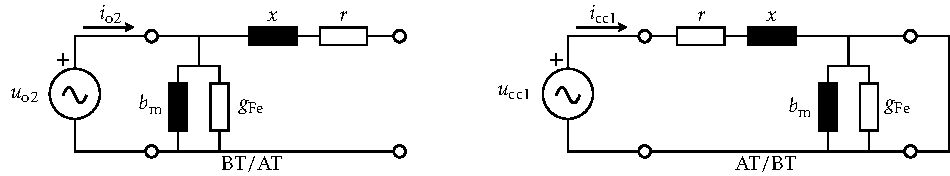
\includegraphics{Imatges/Cap-TrafosPot-Assaig-Buit-CC-Esq-Equiv.pdf}
\caption{Esquemes equivalents d'un transformador en els assajos en
buit i en curt circuit} \label{pic:assaig_buit_cc_esq_equiv}
\end{figure}

Les tensions, els corrents i les pot\`{e}ncies d'aquests dos  assajos,
expressats en p.u. s\'{o}n:
\begin{align}
    u\ped{o2} &=\frac{U\ped{o2}}{U\ped{N2}} &
    i\ped{o2} &=\frac{I\ped{o2}}{I\ped{N2}} &
    w\ped{o}  &=\frac{W\ped{o}}{S\ped{N}} \\[1ex]
    u\ped{cc1} &=\frac{U\ped{cc1}}{U\ped{N1}} &
    i\ped{cc1} &=\frac{I\ped{cc1}}{I\ped{N1}} &
    w\ped{cc} &=\frac{W\ped{cc}}{S\ped{N}}
\end{align}

A partir d'aquests valors podem calcular la imped\`{a}ncia longitudinal
del transformador $\cmplx{z}\ped{cc}=r+\ju x$, i la seva admit\`{a}ncia
transversal $\cmplx{y}\ped{o}=g\ped{Fe}-\ju b\ped{m}$.

\subsubsection{Admit\`{a}ncia transversal}\index{transformadors de pot\`{e}ncia!determinaci\'{o} admit\`{a}ncia transversal}

En l'assaig en buit, el corrent $\cmplx{i}\ped{o2}$ circula
\'{u}nicament per l'admit\`{a}ncia $\cmplx{y}\ped{o}$, i tota la pot\`{e}ncia
$w\ped{o}$ \'{e}s consumida per $g\ped{Fe}$; amb aquestes consideracions
tenim:
\begin{equation}
    g\ped{Fe} = \frac{w\ped{o}}{u\ped{o2}^2} \qquad\qquad
    |\cmplx{y}\ped{o}| = \frac{i\ped{o2}}{u\ped{o2}}
    \qquad\qquad
    b\ped{m} = \sqrt{|\cmplx{y}\ped{o}|^2 - g\ped{Fe}^2}
\end{equation}

Si aquest assaig es fes pel primari, ens quedaria la imped\`{a}ncia
$\cmplx{z}\ped{cc}$ en s\`{e}rie amb l'admit\`{a}ncia $\cmplx{y}\ped{o}$, i
per tant les f\'{o}rmules anteriors no serien correctes, no obstant,
tenint en compte que $|\cmplx{z}\ped{cc}| \ll |1/\cmplx{y}\ped{o}|$,
es  considera que el valor de $\cmplx{z}\ped{cc}$ \'{e}s negligible, i
que les f\'{o}rmules dedu\"{\i}des anteriorment s\'{o}n tamb\'{e} aplicables en
aquests cas, aix\`{o} s\'{\i}, canviant tots els sub\'{\i}ndex {"<}2{">} per {"<}1{">}.

En el cas que l'assaig en buit es faci a tensi\'{o} nominal, tant  si es
fa pel secundari com si es fa pel primari, la tensi\'{o} en buit ser\`{a}
igual a 1 p.u., i per tant es pot ometre el sub\'{\i}ndex {"<}1{">} o {"<}2{">}:
$u\ped{o2} = u\ped{o1} \equiv u\ped{o} = 1$; el mateix passa amb els
sub\'{\i}ndexs del corrent en buit: $i\ped{o2} = i\ped{o1} \equiv
i\ped{o}$. Amb aquestes consideracions tenim:
\begin{equation}
    u\ped{o} = 1 \qquad \Rightarrow \qquad g\ped{Fe} = w\ped{o} \qquad
    |\cmplx{y}\ped{o}| = i\ped{o} \qquad
    b\ped{m} = \sqrt{i\ped{o}^2 - w\ped{o}^2}
    \label{eq:assaig-buit-nomianl}
\end{equation}

\subsubsection{Imped\`{a}ncia longitudinal}\index{transformadors de pot\`{e}ncia!determinaci\'{o} imped\`{a}ncia longitudinal}

En l'assaig en curt circuit, el corrent $\cmplx{i}\ped{cc1}$ circula
\'{u}nicament per la imped\`{a}ncia $\cmplx{z}\ped{cc}$, i tota la pot\`{e}ncia
$w\ped{cc}$ \'{e}s consumida per $r$; amb aquestes consideracions tenim:
\begin{equation}
    r = \frac{w\ped{cc}}{i\ped{cc1}^2} \qquad\qquad
    |\cmplx{z}\ped{cc}| = \frac{u\ped{cc1}}{i\ped{cc1}} \qquad\qquad
    x = \sqrt{|\cmplx{z}\ped{cc}|^2 - r^2}
\end{equation}

Si aquest assaig es fes pel secundari, ens quedaria la imped\`{a}ncia
$\cmplx{z}\ped{cc}$ en para{\l.l}el amb l'admit\`{a}ncia
$\cmplx{y}\ped{o}$, i per tant les f\'{o}rmules anteriors no serien
correctes, no obstant, tenint en compte que $|\cmplx{y}\ped{o}| \ll
|1/\cmplx{z}\ped{cc}|$, es considera que el valor de
$\cmplx{y}\ped{o}$ \'{e}s negligible, i que les f\'{o}rmules dedu\"{\i}des
anteriorment s\'{o}n tamb\'{e} aplicables en aquests cas, aix\`{o} s\'{\i}, canviant
tots els sub\'{\i}ndex {"<}1{">} per {"<}2{">}.

En el cas que l'assaig en curt circuit es faci a corrent nominal,
tant  si es fa pel primari  com si es fa pel secundari, el corrent
de curt circuit ser\`{a} igual a 1 p.u., i per tant es pot ometre el
sub\'{\i}ndex {"<}1{">} o {"<}2{">}: $i\ped{cc1} = i\ped{cc2} \equiv i\ped{cc} = 1$;
el mateix passa amb els sub\'{\i}ndexs de la tensi\'{o} de curt circuit:
$u\ped{cc1} = u\ped{cc2} \equiv u\ped{cc}$. En aquest cas, el valor
de $u\ped{cc}$, tamb\'{e} es coneix amb la denominaci\'{o} de
tensi\'{o} relativa de curt  circuit en tant per u, utilitzant-se  el
s\'{\i}mbol $\varepsilon\ped{cc}$; per a $r$ i $x$ s'utilitzen tamb\'{e} els
s\'{\i}mbols $\varepsilon\ped{rcc}$ i $\varepsilon\ped{xcc}$
respectivament. Amb aquestes consideracions tenim:
\begin{equation}
    i\ped{cc} = 1 \qquad \Rightarrow \qquad r \equiv \varepsilon\ped{rcc} = w\ped{cc} \qquad
    |\cmplx{z}\ped{cc}| \equiv \varepsilon\ped{cc} = u\ped{cc} \qquad
    x \equiv \varepsilon\ped{xcc} = \sqrt{u\ped{cc}^2 - w\ped{cc}^2}
    \label{eq:assaig-cc-nomianl}
\end{equation}

Si es desitja utilitzar l'esquema equivalent redu\"{\i}t en {"<}T{">} de la Figura \vref{pic:tr-pot-esquema-equiv-reduit-T} es poden utilitzar amb prou aproximaci\'{o} les relacions seg\"{u}ents:
\begin{equation}
    r_1 = r_2 = \frac{r}{2} \qquad\qquad x\ped{d1} = x\ped{d1} = \frac{x}{2}
\end{equation}


\begin{exemple}
    Tenim un transformador monof\`{a}sic amb les seg\"{u}ents caracter\'{\i}stiques:
    \[S\ped{N}=400\unit{kVA},\,U\ped{N1}=25\unit{kV},\, U\ped{N2}=400\unit{V},\, \varepsilon\ped{cc}=0{,}04,\, W\ped{cc}=4\unit{kW},\, i\ped{o}=0{,}02,\,  W\ped{o}=2\unit{kW}\]
     El transformador t\'{e} connectada una c\`{a}rrega en el secundari que consumeix $200\unit{kW}$ amb $\cos{\varphi}=0{,}8\text{(i)}$; en aquestes condicions la tensi\'{o} secund\`{a}ria \'{e}s de $380\unit{V}$.
    Es tracta de trobar en primer lloc els par\`{a}metres del transformador, i a continuaci\'{o} la tensi\'{o} prim\`{a}ria, la caiguda de tensi\'{o} referida al secundari i el rendiment.

    Comen\c{c}arem per trobar els par\`{a}metres del transformador en p.u., utilitzant els valors base propis del transformadors, als quals estan referits $\varepsilon\ped{cc}$ i $i\ped{o}$, \'{e}s a dir:
    \[ S\ped{B}=400\unit{kVA},\quad U\ped{B1}=25\unit{kV},\quad U\ped{B2}=400\unit{V}\]

    Donat que no es diu el contrari suposarem que l'assaig en buit s'ha realitzat aplicant la tensi\'{o} nominal al secundari (BT) i deixant obert el primari (AT), i que l'assaig en curt circuit s'ha fet fent circular el corrent nominal pel primari (AT) tot curtcircuitant el secundar (BT). En aquestes condicions, podem aplicar les equacions \eqref{eq:assaig-buit-nomianl} i \eqref{eq:assaig-cc-nomianl}:
   \begin{align*}
        g\ped{Fe} &= w\ped{o} = \frac{2\unit{kW}}{400\unit{kVA}} = 0{,}005 \\
        |\cmplx{y}\ped{o}| &= i\ped{o}  = 0{,}02 \\
        b\ped{m} &= \sqrt{i\ped{o}^2 - w\ped{o}^2} = \sqrt{0{,}02^2 - 0{,}005^2} = 0{,}0194\\
        r &= w\ped{cc} = \frac{4\unit{kW}}{400\unit{kVA}} = 0{,}01 \\
        |\cmplx{z}\ped{cc}| &=  \varepsilon\ped{cc} = 0{,}04 \\
        x &= \sqrt{\varepsilon\ped{cc}^2 - w\ped{cc}^2} = \sqrt{0{,}04^2-0{,}01^2} = 0{,}0387
  \end{align*}

        A continuaci\'{o}, convertim la pot\`{e}ncia absorbida per la c\`{a}rrega i la tensi\'{o} secund\`{a}ria, la qual prendrem com a refer\`{e}ncia d'angles,  a valors expressats en p.u.:
  \begin{align*}
    \cmplx{s}_2 &= \frac{200\unit{kW}}{400\unit{kVA}} + \ju \frac{200\cdot \frac{\sqrt{1-0{,}8^2}}{0{,}8}\unit{kVAr}}{400\unit{kVA}} = 0{,}5 + \ju 0{,}375\\[1ex]
    \cmplx{u}_2 &= \frac{380\unit{V}}{400\unit{V}} = 0{,}95
  \end{align*}

    Amb aquests valors ens queda l'esquema seg\"{u}ent:

    \begin{figure}[htb]
    \centering
        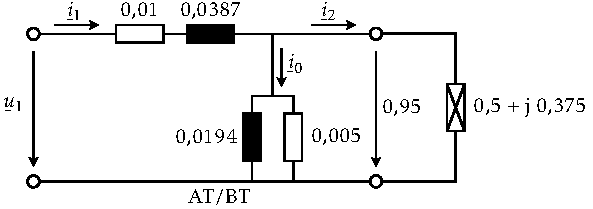
\includegraphics{Imatges/Cap-TrafosPot-Exemple-TR.pdf}
    \end{figure}

    Calculem ara $\cmplx{i}_2$, $\cmplx{i}_0$, $\cmplx{i}_1$ i $\cmplx{u}_1$:
    \begin{align*}
    \cmplx{i}_2 &= \frac{\cmplx{s}_2^*}{\cmplx{u}_2^*} = \frac{0{,}5 - \ju 0{,}375}{0{,}95} = 0{,}6579_{\measuredangle -36{,}87\degree} \\[1ex]
    \cmplx{i}_0 &= \cmplx{u}_2 (g\ped{Fe}-\ju b\ped{m}) = 0{,}95\cdot(0{,}005-\ju 0{,}0194) = 0{,}0190_{\measuredangle -75{,}55\degree} \\[1ex]
    \cmplx{i}_1 &= \cmplx{i}_2 + \cmplx{i}_0 =0{,}6579_{\measuredangle -36{,}87\degree} +0{,}0190_{\measuredangle -75{,}55\degree} = 0{,}6728_{\measuredangle -37{,}88\degree} \\[1ex]
    \cmplx{u}_1 &=(r+\ju x) \cmplx{i}_1 + \cmplx{u}_2 = (0{,}01+\ju 0{,}0387) \cdot 0{,}6728_{\measuredangle -37{,}88\degree} + 0{,}95 = 0{,}9715_{\measuredangle 0{,}97\degree}
  \end{align*}

  La tensi\'{o} prim\`{a}ria expressada en volt val:
  \[
    \cmplx{U}_1 = 0{,}9715_{\measuredangle 0{,}97\degree}\cdot 25\unit{kV} = 24287{,}5_{\measuredangle 0{,}97\degree}\unit{V}
  \]

   La caiguda de tensi\'{o} \'{e}s:
   \[
        \Delta u = |\cmplx{u}_1| - |\cmplx{u}_2| = 0{,}9715 - 0{,}95 = 0{,}0215
   \]

   Aquest valor referit al secundari val:
   \[
        \Delta U_2 = 0{,}0215\cdot 400\unit{V} = 8{,}6\unit{V}
   \]

   Calculem finalment el rendiment el transformador, a partir de les p\`{e}rdues en el coure  i en el ferro:
   \begin{align*}
    p\ped{Cu} &= r |\cmplx{i}_1|^2  = 0{,}01\cdot 0{,}6728^2 = 0{,}004527\\
    p\ped{Fe} &= g\ped{Fe} |\cmplx{u}_2|^2 = 0{,}005\cdot 0{,}95^2 = 0{,}004513\\
    \eta &= \frac{p_2}{p_2 + p\ped{Cu} + p\ped{Fe}} = \frac{0{,}5}{0{,}5 + 0{,}004527 + 0{,}004513 } = 0{,}98
  \end{align*}

\end{exemple}

\section{Transformadors de tres debanats}\index{transformadors de pot\`{e}ncia!de tres debanats}

Un transformador de tres debanats est\`{a} format per un debanat primari i dos debanats secundaris; la pot\`{e}ncia del debanat primari es reparteix entre els dos secundaris, les tensions dels quals poden ser iguals o diferents.

Anomenant al primari {"<}P{">}, a un secundari {"<}S{">} i a l'altre {"<}T{">} (terciari), l'esquema equivalent redu\"{\i}t d'un transformador de tres debanats, tenint en compte nom\'{e}s les imped\`{a}ncies longitudinals,  \'{e}s el representat en la Figura \vref{pic:trafo-3-deban}.

\begin{figure}[htb]
\centering
    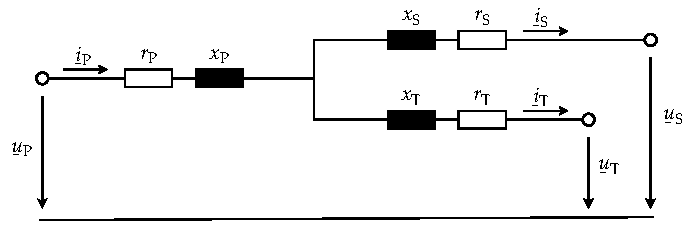
\includegraphics{Imatges/Cap-TrafosPot-3-debanats.pdf}
\caption{Esquema equivalent redu\"{\i}t d'un transformador de tres debanats}
\label{pic:trafo-3-deban}
\end{figure}

Com en el cas dels transformadors de dos debanats, han d'escollir-se tensions base proporcionals a les tensions nominals dels tres debanats i una pot\`{e}ncia base \'{u}nica.

Les tres imped\`{a}ncies d'aquest circuit $\cmplx{z}\ped{P} = r\ped{P} + \ju x\ped{P}$, $\cmplx{z}\ped{S} = r\ped{S} + \ju x\ped{S}$ i $\cmplx{z}\ped{T} = r\ped{T} + \ju x\ped{T}$ es calculen a partir de les imped\`{a}ncies entre parells de debanats $\cmplx{z}\ped{PS}$, $\cmplx{z}\ped{PT}$ i $\cmplx{z}\ped{ST}$, que s\'{o}n les que s'obtenen dels assajos del transformador:
\begin{subequations}
\begin{align}
    \cmplx{z}\ped{P} &= \frac{\cmplx{z}\ped{PS}+\cmplx{z}\ped{PT}-\cmplx{z}\ped{ST}}{2}  \\[1ex]
    \cmplx{z}\ped{S} &= \frac{\cmplx{z}\ped{PS}+\cmplx{z}\ped{ST}-\cmplx{z}\ped{PT}}{2}  \\[1ex]
    \cmplx{z}\ped{T} &= \frac{\cmplx{z}\ped{PT}+\cmplx{z}\ped{ST}-\cmplx{z}\ped{PS}}{2}
\end{align}
\end{subequations}

En aquestes equacions cal tenir en compte que les tres imped\`{a}ncies $\cmplx{z}\ped{PS}$, $\cmplx{z}\ped{PT}$ i $\cmplx{z}\ped{ST}$ han d'estar donades en p.u. referides a un base com\'{u}, o han d'estar donades en ohm referides a un mateix debanat. Cal dir a m\'{e}s, que el punt d'uni\'{o} de les tres imped\`{a}ncies $\cmplx{z}\ped{P}$, $\cmplx{z}\ped{S}$ i $\cmplx{z}\ped{T}$ no te res a veure amb el neutre del sistema, i que aquestes imped\`{a}ncies calculades poden tenir valors  negatius.

\begin{exemple}
    Tenim un transformador de tres debanats amb les seg\"{u}ents caracter\'{\i}stiques: primari de 15\unit{MVA} i 66\unit{kV}, secundari de 10\unit{MVA} i 13,2\unit{kV} i terciari de 5\unit{MVA} i 2,3\unit{kV}; les imped\`{a}ncies entre debanats s\'{o}n: $\cmplx{z}\ped{PS} = \ju 0{,}07$ (referida a 15\unit{MVA} i 66\unit{kV}/13,2\unit{kV}), $\cmplx{z}\ped{PT} = \ju 0{,}09$ (referida a 15\unit{MVA} i 66\unit{kV}/2,3\unit{kV}) i $\cmplx{z}\ped{ST} = \ju 0{,}08$ (referida a 10\unit{MVA} i 13,2\unit{kV}/2,3\unit{kV}).  Es tracta de calcular les imped\`{a}ncies del circuit equivalent redu\"{\i}t expressades en ohm en el primari, i expressades en p.u. en una base de 30\unit{MVA} i 66\unit{kV}/13,2\unit{kV}/2,3\unit{kV}.

    Comencem calculant les imped\`{a}ncies en ohm referides al primari, convertint en primer lloc els tres valors $\cmplx{z}\ped{PS}$, $\cmplx{z}\ped{PT}$ i $\cmplx{z}\ped{ST}$ a valors \`{o}hmics $\cmplx{z}\ped{PS}'$, $\cmplx{z}\ped{PT}'$ i $\cmplx{z}\ped{ST}'$ referits a aquest debanat. Per obtenir $\cmplx{z}\ped{PS}'$ i $\cmplx{z}\ped{PT}'$ nom\'{e}s cal multiplicar aquests valors per la imped\`{a}ncia base del primari; en el cas de $\cmplx{z}\ped{ST}'$ s\'{o}n necessaris dos passos, primer multipliquem per la imped\`{a}ncia base del secundari, amb la qual cosa tindrem una imped\`{a}ncia $\cmplx{z}\ped{ST}''$ referida al secundari,  i despr\'{e}s multipliquem per la relaci\'{o} de transformaci\'{o} entre primari i secundari al quadrat:
    \begin{align*}
        \cmplx{z}\ped{PS}' &=  \ju 0{,}07 \cdot \frac{(66\unit{kV})^2}{15\unit{MVA}} = \ju 20{,}328\unit{\ohm}\\
        \cmplx{z}\ped{PT}' &=  \ju 0{,}09 \cdot \frac{(66\unit{kV})^2}{15\unit{MVA}} = \ju 26{,}136\unit{\ohm}\\
        \cmplx{z}\ped{ST}'' &=  \ju 0{,}08 \cdot \frac{(13{,}2\unit{kV})^2}{10\unit{MVA}} = \ju 1{,}39392\unit{\ohm}\\
        \cmplx{z}\ped{ST}' &=  1{,}39392\unit{\ohm} \cdot {\left(\frac{66\unit{kV}}{13{,}2\unit{kV}}\right)}^2 = \ju 34{,}848\unit{\ohm}
    \end{align*}

    Els valors buscats $\cmplx{z}\ped{P}'$, $\cmplx{z}\ped{S}'$ i $\cmplx{z}\ped{T}'$ s\'{o}n:
    \begin{align*}
        \cmplx{z}\ped{P}' &=  \frac{\ju 20{,}328\unit{\ohm} + \ju 26{,}136\unit{\ohm} - \ju 34{,}848\unit{\ohm}}{2} = \ju 5{,}808\unit{\ohm} \\[1ex]
        \cmplx{z}\ped{S}' &=  \frac{\ju 20{,}328\unit{\ohm} + \ju 34{,}848\unit{\ohm} - \ju 26{,}136\unit{\ohm}}{2} = \ju 14{,}520\unit{\ohm} \\[1ex]
        \cmplx{z}\ped{T}' &=  \frac{\ju 26{,}136\unit{\ohm} + \ju 34{,}848\unit{\ohm} - \ju 20{,}328\unit{\ohm}}{2} = \ju 20{,}328\unit{\ohm}
    \end{align*}

    Calculem ara els valors de les imped\`{a}ncies en p.u. en la base demanada, convertint en primer lloc els tres valors $\cmplx{z}\ped{PS}$, $\cmplx{z}\ped{PT}$ i $\cmplx{z}\ped{ST}$ a aquesta base; nom\'{e}s caldr\`{a} fer una conversi\'{o} de pot\`{e}ncies ja que les tensions s\'{o}n les mateixes:
    \begin{align*}
        \cmplx{z}\ped{PS} &=  \ju 0{,}07 \cdot \frac{30\unit{MVA}}{15\unit{MVA}} = \ju 0{,}14\\[1ex]
        \cmplx{z}\ped{PT} &=  \ju 0{,}09 \cdot \frac{30\unit{MVA}}{15\unit{MVA}} = \ju 0{,}18\\[1ex]
        \cmplx{z}\ped{ST} &=  \ju 0{,}08 \cdot \frac{30\unit{MVA}}{10\unit{MVA}} = \ju 0{,}24
    \end{align*}

    Els valors buscats $\cmplx{z}\ped{P}$, $\cmplx{z}\ped{S}$ i $\cmplx{z}\ped{T}$ s\'{o}n:
    \begin{align*}
        \cmplx{z}\ped{P} &=  \frac{\ju 0{,}14 + \ju 0{,}18 - \ju 0{,}24}{2} = \ju 0{,}04 \\[1ex]
        \cmplx{z}\ped{S} &=  \frac{\ju 0{,}14 + \ju 0{,}24 - \ju 0{,}18}{2} = \ju 0{,}10 \\[1ex]
        \cmplx{z}\ped{T} &=  \frac{\ju 0{,}18 + \ju 0{,}24 - \ju 0{,}14}{2} = \ju 0{,}14
    \end{align*}

     Com \'{e}s natural, si multipliquem aquests valors en p.u.  $\cmplx{z}\ped{P}$, $\cmplx{z}\ped{S}$ i $\cmplx{z}\ped{T}$ per la imped\`{a}ncia base del primari $\frac{(66\unit{kV})^2}{30\unit{MVA}}=145{,}2\unit{\ohm}$, obtindrem els valors \`{o}hmics $\cmplx{z}\ped{P}'$,     $\cmplx{z}\ped{S}'$ i $\cmplx{z}\ped{T}'$ que hem calculat anteriorment.

\end{exemple}


\section{Caracter\'{\i}stiques particulars  dels transformadors trif\`{a}sics}

\subsection{Tipus de connexions}\index{transformadors de pot\`{e}ncia!trif\`{a}sics!tipus de connexions}

Connectant tres transformador monof\`{a}sics entre s\'{\i}, podem crear-ne un de trif\`{a}sic (banc trif\`{a}sic). No obstant, \'{e}s m\'{e}s com\'{u} construir els transformadors trif\`{a}sics d'una sola pe\c{c}a, ja sigui amb un nucli de tres columnes (transformador de columnes) o amb un nucli de cinc columnes (transformador cuirassat).

Tant el primari com el secundari poden connectar-se de tres maneres diferents, en estrella (Y) en triangle (D) o en ziga-zaga (Z); las caracter\'{\i}stiques principals de cadascuna d'aquestes connexions s\'{o}n:

\begin{dinglist}{'167}
   \item \textbf{Y}. La connexi\'{o} en estrella permet tenir el neutre accessible. El corrent de l\'{\i}nia \'{e}s el que circula per cada debanat; cada debanat suporta la tensi\'{o} senzilla. No t\'{e} un bon comportament amb c\`{a}rregues desequi{\l.l}ibrades.
   \item \textbf{D}. La connexi\'{o} en triangle no pot proporcionar un neutre. El corrent que circula per cada debanat \'{e}s el de l\'{\i}nia dividit per $\sqrt{3}$; cada debanat suporta la tensi\'{o} composta. Per una mateixa tensi\'{o} i pot\`{e}ncia, els debanats d'un transformador connectat en triangle han de tenir $\sqrt{3}$ vegades m\'{e}s espires que els d'un transformador connectat en estrella; la quantitat de coure no obstant, pot ser la mateixa, ja que la secci\'{o} pot ser menor, donat que el corrent que circula pels debanats \'{e}s $\sqrt{3}$ vegades menor. T\'{e} un bon comportament amb c\`{a}rregues desequi{\l.l}ibrades ja que redistribueix parcialment el desequ{\l.l}ibri entre les fases.
   \item \textbf{Z}. La connexi\'{o} en ziga-zaga permet tenir el neutre accessible, per\`{o} requereix dues bobines iguals per fase. El corrent que circula per cada debanat \'{e}s el de l\'{\i}nia; cadascuna de les dues bobines d'un debanat suporta la tensi\'{o} composta dividida per 3; aquestes dues tensions no estan en fase i la seva suma \'{e}s igual a la tensi\'{o} senzilla. Per una mateixa tensi\'{o} i pot\`{e}ncia, els debanats d'un transformador connectat en ziga-zaga han de tenir $2/\sqrt{3}$ vegades m\'{e}s espires que els d'un transformador connectat en estrella; la quantitat de coure \'{e}s m\'{e}s gran ja que la secci\'{o} ha de mantenir-se igual, donat que el corrent que circula pels debanats \'{e}s el mateix. T\'{e} un bon comportament amb c\`{a}rregues desequi{\l.l}ibrades.
\end{dinglist}

Les combinacions possibles de connexions de primari i secundari s\'{o}n moltes, per\`{o} nom\'{e}s s'utilitzen les seg\"{u}ents:
\begin{dinglist}{'167}
   \item \textbf{Estrella--Estrella}. \'{E}s poc utilitzada ja que no es comporta b\'{e} amb c\`{a}rregues desequi{\l.l}ibrades, originant despla\c{c}aments dels neutres o deformacions de les ones de tensi\'{o}. Aquest comportament millora connectant el neutre del primari a terra.
   \item \textbf{Triangle--Estrella}. S\'{o}n molt utilitzats con a transformadors de distribuci\'{o} degut a la accessibilitat del neutre i perqu\`{e} admeten tot tipus de c\`{a}rregues desequi{\l.l}ibrades. Tamb\'{e} s\'{o}n \'{u}tils com a transformadors elevadors de principi de l\'{\i}nia.
   \item \textbf{Estrella--Triangle}. S\'{o}n \'{u}tils com a transformadors reductors al final de l\'{\i}nia.
   \item \textbf{Triangle--Triangle}. Es comportem b\'{e} amb c\`{a}rregues desequi{\l.l}ibrades, per\`{o} l'abs\`{e}ncia de neutre pot ser un inconvenient si es volent utilitzar per distribuci\'{o}.
   \item \textbf{Triangle--Ziga-zaga i Estrella--Ziga-zaga}. S\'{o}n bastant utilitzats en distribuci\'{o} de baixa pot\`{e}ncia, degut al seu bon comportament amb c\`{a}rregues desequi{\l.l}ibrades, La connexi\'{o} ziga-zaga es troba sempre en el costat de baixa tensi\'{o}, per la possibilitat que t\'{e} de crear un neutre artificial.
   \item \textbf{Estrella--Estrella--Triangle} Permet tenir accessible ambd\'{o}s  neutres i tolera  b\'{e} les c\`{a}rregues  desequi{\l.l}ibrades. El debanat en triangle (terciari) no acostuma a tenir c\`{a}rrega i s'utilitza per eliminar fluxos homopolars. S'utilitza per interconnectar sistemes d'alta tensi\'{o}.
\end{dinglist}


\subsection{\'{I}ndex horari i grup de connexi\'{o}}\label{sec:connex-index-horari}\index{transformadors de pot\`{e}ncia!trif\`{a}sics!\'{\i}ndex horari}\index{transformadors de pot\`{e}ncia!trif\`{a}sics!grup de connexi\'{o}}

En un transformador monof\`{a}sic el desfase entre tensi\'{o} prim\`{a}ria i secund\`{a}ria nom\'{e}s pot ser $0\unit{\degree}$ o $180\unit{\degree}$; el mateix passa amb els corrents. En canvi, en el cas de transformadors trif\`{a}sics hi ha m\'{e}s desfases possibles, depenent del tipus de connexi\'{o}; el desfase \'{e}s sempre m\'{u}ltiples de $30\unit{\degree}$ ($\frac{\piup}{6}\unit{rad}$).

L'\'{\i}ndex horari \'{e}s l'angle entre una magnitud  prim\`{a}ria (tensi\'{o} o corrent) i la magnitud secund\`{a}ria corresponent, per exemple entre $\cmplx{U}\ped{AB}$ i $\cmplx{U}\ped{ab}$, o entre $\cmplx{U}\ped{AN}$ i $\cmplx{U}\ped{an}$.

L'\'{\i}ndex horari es refereix a un transformador alimentat pel costat de tensi\'{o} m\'{e}s alta  amb un sistema trif\`{a}sic sim\`{e}tric de seq\"{u}\`{e}ncia directa. Donat que els desfase possibles s\'{o}n m\'{u}ltiples de $30\unit{\degree}$, hi ha dotze casos possibles, aix\`{o} ha fet que es cre\"{\i} l'analogia d'un rellotge: la busca dels minuts es co{\l.l}oca a les dotze, representant una tensi\'{o} del costat de tensi\'{o} m\'{e}s alta, i la busca de les hores, representant la tensi\'{o} corresponent del costat de tensi\'{o} m\'{e}s baixa, es co{\l.l}oca amb l'angle corresponent. Per exemple, si la tensi\'{o} del costat de tensi\'{o} m\'{e}s baixa queda a les cinc, aix\`{o} ens indica que aquesta tensi\'{o} retarda $5\cdot 30\unit{\degree}= 150\unit{\degree}$ a la corresponent del costat de tensi\'{o} m\'{e}s alta.

L'\'{\i}ndex horari ens indica de fet, l'angle de retard de la tensi\'{o} del costat de tensi\'{o} m\'{e}s baixa respecte del costat de tensi\'{o} m\'{e}s alta, quan el transformador es troba en buit.

Normalment no \'{e}s necessari tenir en compte l'\'{\i}ndex horari en els c\`{a}lculs, ja que no cal con\`{e}ixer el desfase real entre magnituds prim\`{a}ries i secund\`{a}ries; quan aix\`{o} sigui necessari es poden fer els c\`{a}lculs de la manera usual sense tenir en compte l'\'{\i}ndex horari, i afegir el desfase posteriorment. Si $h$ \'{e}s l'\'{\i}ndex horari (entre 0 i 11), la relaci\'{o} entre l'angle d'una magnitud del costat de tensi\'{o} m\'{e}s alta $\varphi\ped{AT}$ i l'angle de la magnitud corresponent del costat de tensi\'{o} m\'{e}s baixa $\varphi\ped{BT}$ \'{e}s:
\begin{equation}
    \varphi\ped{AT} = \varphi\ped{BT} + h\frac{\piup}{6}\label{eq:fi-AT-BT}
\end{equation}


A partit del tipus de connexi\'{o} del primari i del secundari en estrella (Y), triangle (D) o ziga-zaga (Z), i de l'\'{\i}ndex horari, queda definit el grup de connexi\'{o} del transformador; normalment est\`{a} format per dues lletres i un n\'{u}mero:
\begin{dingautolist}{'312}
   \item La primera lletra, escrita en maj\'{u}scula, indica la connexi\'{o} del debanat de tensi\'{o} m\'{e}s alta, independentment de si \'{e}s el primari o el secundari.
   \item La segona lletra, escrita en min\'{u}scula, indica la connexi\'{o} del debanat de tensi\'{o} m\'{e}s baixa.
   \item Un n\'{u}mero al final indica l'\'{\i}ndex horari (entre 0 i 11).
\end{dingautolist}

Una nomenclatura m\'{e}s completa afegeix la lletra {"<}N{">} o {"<}n{">} despr\'{e}s de la lletra del debanat corresponent, si el neutre \'{e}s f\'{\i}sicament accessible, per exemple Dyn11 o YNd6.

\begin{exemple}
    Es tracte de deduir l'\'{\i}ndex horari de dos transformador a partir de les seves connexions.

    El primer transformador \'{e}s del tipus Yz. Per tal de deduir el seu \'{\i}ndex horari, compararem les tensions
    $\cmplx{U}\ped{AN}$ i $\cmplx{U}\ped{an}$. Comencem dibuixant les tres tensions fase--neutre $\cmplx{U}\ped{AN}$, $\cmplx{U}\ped{BN}$ i $\cmplx{U}\ped{CN}$. Donat que $\cmplx{U}\ped{an} = \cmplx{U}\ped{aa'} + \cmplx{U}\ped{a'n}$, dibuixem primer la tensi\'{o} $\cmplx{U}\ped{aa'}$, que est\`{a} en fase amb la tensi\'{o} $\cmplx{U}\ped{AN}$, i a continuaci\'{o} la tensi\'{o} $\cmplx{U}\ped{na'}$, que est\`{a} en fase amb la tensi\'{o} $\cmplx{U}\ped{BN}$; un cop tenim situats els punts a i n, ja podem dibuixar la tensi\'{o} $\cmplx{U}\ped{an}$. Dibuixant ara juntes $\cmplx{U}\ped{AN}$ i $\cmplx{U}\ped{an}$  veiem que l'\'{\i}ndex horari \'{e}s 11.

    \begin{figure}[!h]
    \centering
        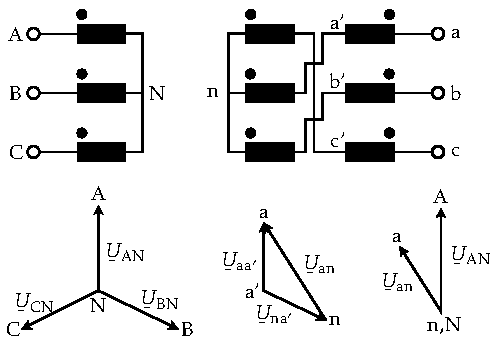
\includegraphics{Imatges/Cap-TrafosPot-Exemple-Yz.pdf}
    \end{figure}

     El segon transformador \'{e}s del tipus Dyn. Per tal de deduir el seu \'{\i}ndex horari, compararem com en el cas anterior, les tensions $\cmplx{U}\ped{AN}$ i $\cmplx{U}\ped{an}$. Comencem dibuixant les tres tensions fase--neutre $\cmplx{U}\ped{AN}$, $\cmplx{U}\ped{BN}$ i $\cmplx{U}\ped{CN}$ i la tensi\'{o} fase--fase $\cmplx{U}\ped{AB}$.  A continuaci\'{o} dibuixem la tensi\'{o} $\cmplx{U}\ped{na}$, que est\`{a} en fase amb la tensi\'{o} $\cmplx{U}\ped{AB}$; Dibuixant ara juntes $\cmplx{U}\ped{AN}$ i $\cmplx{U}\ped{an}$ (mateixa orientaci\'{o} que $\cmplx{U}\ped{na}$ per\`{o} sentit contrari),  veiem que l'\'{\i}ndex horari \'{e}s 5.

    \begin{figure}[!h]
    \centering
        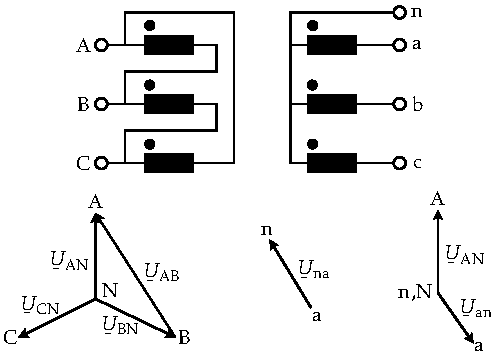
\includegraphics{Imatges/Cap-TrafosPot-Exemple-Dy.pdf}
    \end{figure}
\end{exemple}

El desfase introdu\"{\i}t per l'\'{\i}ndex horari es pot modelar si es vol, com un transformador ideal amb relaci\'{o} de transformaci\'{o} complexa. En el cas de l'esquema equivalent de la Figura  \vref{pic:tr-pot-esquema-equiv}, el transformador all\'{\i} dibuixat
se substitueix per un de relaci\'{o} $\cmplx{m}:1$. En el cas dels esquemes equivalents redu\"{\i}ts en {"<}T{">} de la Figura \vref{pic:tr-pot-esquema-equiv-reduit-T} i en {"<}L{">} de la Figura \vref{pic:tr-pot-esquema-equiv-reduit-L}, cal afegir un transformador ideal de relaci\'{o} de transformaci\'{o}  $\cmplx{m}\ped{r}:1$; aquest transformador pot afegir-se indistintament  al principi o al final de l'esquema equivalent redu\"{\i}t, ja que es compleix $|\cmplx{m}\ped{r}|=1$.

A partir de l'\'{\i}ndex horari $h$ i depenent de si el primari \'{e}s el costat de tensi\'{o} m\'{e}s alta o el de tensi\'{o} m\'{e}s baixa, tenim:
\begin{equation}
\begin{array}{c}\text{Transformador}\\
\text{AT/BT}
\end{array} \left\{
\begin{array}{l}
   \cmplx{m} = (U\ped{N1}/U\ped{N2})_{\measuredangle h \frac{\piup}{6}} \\[2.7ex]
   \cmplx{m}\ped{r} = 1_{\measuredangle h\frac{\piup}{6}}
\end{array}
\right. \qquad
\begin{array}{c}\text{Transformador}\\
\text{BT/AT}
\end{array} \left\{
\begin{array}{l}
   \cmplx{m} = (U\ped{N1}/U\ped{N2})_{\measuredangle -h \frac{\piup}{6}} \\[2.7ex]
   \cmplx{m}\ped{r} = 1_{\measuredangle -h\frac{\piup}{6}}
\end{array}
\right.
\label{eq:rel-transf-cmplx}
\end{equation}

Cal tenir en compte que les equacions \eqref{eq:rel-transf-cmplx}, aix\'{\i} com l'equaci\'{o} \eqref{eq:fi-AT-BT}, s\'{o}n v\`{a}lides quan tenim un sistema directe de tensions trif\`{a}siques; en el cas que tingu\'{e}ssim un sistema invers de tensions trif\`{a}siques, caldria canviar el signe del desfase introdu\"{\i}t per l'\'{\i}ndex horari, en totes les equacions mencionades.

La relaci\'{o} entre les tensions i corrents de primari i secundari d'aquests transformadors ideals \'{e}s:
\begin{subequations}
\begin{align}
    \cmplx{U}_1 &= \cmplx{m} \cmplx{U}_2 &  \cmplx{I}_1 &= \frac{\cmplx{I}_2}{\cmplx{m}^*} \\[0.5ex]
   \cmplx{u}_1 &= \cmplx{m}\ped{r} \cmplx{u}_2 &  \cmplx{i}_1 &= \frac{\cmplx{i}_2}{\cmplx{m}\ped{r}^*}
\end{align}
\end{subequations}

\begin{exemple}
    Tenim un transformador Dy9, on el primari \'{e}s el costat de tensi\'{o} m\'{e}s alta i el secundari el de tensi\'{o} m\'{e}s baixa; la tensi\'{o} secund\`{a}ria calculada sense tenir en compte l'\'{\i}ndex horari val $0{,}95_{\measuredangle -17\degree}\unit{p.u.}$ Es tracta de trobar l'angle real d'aquesta tensi\'{o} tenint en compte l'\'{\i}ndex horari.

    Donat que es tracta d'un transformador AT/BT, tenim:
    \[\cmplx{m}\ped{r} = 1_{\measuredangle 9\cdot\frac{\piup}{6}} = 1_{\measuredangle 270\degree}\]
     Per tant, la tensi\'{o} secund\`{a}ria real \'{e}s:
    \[\cmplx{u}_2 = \frac{\cmplx{u}_1}{\cmplx{m}\ped{r}} = \frac{0{,}95_{\measuredangle -17\degree}}{1_{\measuredangle 270\degree}} = 0{,}95_{\measuredangle -287\degree} = 0{,}95_{\measuredangle 73\degree} \]
\end{exemple}



\section{\texorpdfstring{Connexi\'{o} de transformadors en para{\l.l}el}{Connexi\'{o} de transformadors en paral-lel}}\index{transformadors de pot\`{e}ncia!connexi\'{o} en para{\l.l}el}

El que s'explica a continuaci\'{o} \'{e}s v\`{a}lid per a transformadors
monof\`{a}sics i trif\`{a}sics; com \'{e}s habitual, en el cas dels
transformadors trif\`{a}sics, les tensions nominals s\'{o}n les tensions
fase--fase, i la pot\`{e}ncia nominal \'{e}s la pot\`{e}ncia trif\`{a}sica.

\subsection{Condicions m\'{\i}nimes de connexi\'{o}}\index{transformadors de pot\`{e}ncia!connexi\'{o} en para{\l.l}el!condicions m\'{\i}nimes}

Les condiciones m\'{\i}nimes que han de complir dos transformadors A i B per poder ser connectats en para{\l.l}el, \'{e}s tenir la mateixa relaci\'{o} de transformaci\'{o} (no cal que les tensions nominals siguin iguals, encara que s\'{\i} que han de ser properes), i en el cas de transformadors trif\`{a}sics, tenir a m\'{e}s el mateix \'{\i}ndex horari:
\begin{align}
    m\ped{A} &= m\ped{B}\\
    h\ped{A} &= h\ped{B}
\end{align}

La condici\'{o} $m\ped{A} = m\ped{B}$ \'{e}s necess\`{a}ria per evitar circulaci\'{o} de corrent entre els dos transformadors connectats en para{\l.l}el. Si $m\ped{A} \neq m\ped{B}$, utilitzant el circuit equivalent  Th\'{e}venin vist des del secundari de ambd\'{o}s transformadors, dedu\"{\i}t en la secci\'{o} \vref{sec:trafo-thevenin}, podem obtenir el corrent $\cmplx{I}\ped{circ}^{''}$ que circula del transformador A cap al B , estant els secundaris en buit, a partir de les imped\`{a}ncies i tensions Th\'{e}venin dels dos transformadors:
\begin{equation}
    \cmplx{I}\ped{circ}^{''} = \frac{\cmplx{U}\ped{Th,A}^{''}-\cmplx{U}\ped{Th,B}^{''}}{\cmplx{Z}\ped{Th,A}^{''}+\cmplx{Z}\ped{Th,B}^{''}}
\end{equation}

Pel que fa als \'{\i}ndexs horaris, no cal de fet que siguin estrictament iguals, n'hi ha prou amb que els \'{\i}ndexs siguin compatibles, \'{e}s a dir que variant les connexions externes es puguin obtenir dos \'{\i}ndexs iguals; aix\`{o} \'{e}s possible quan els dos \'{\i}ndexs difereixen en $120\degree$ o en $240\degree$, o quan s\'{o}n sim\`{e}trics respecte les 12, com per exemple 1 i 11 o 5 i 7.

\begin{exemple}
    En la figura seg\"{u}ent es pot veure com han de connectar-se en para{\l.l}el tres transformador amb grups de connexi\'{o} Dy1, Dy5 i Dy11.

    \begin{figure}[h]
    \centering
        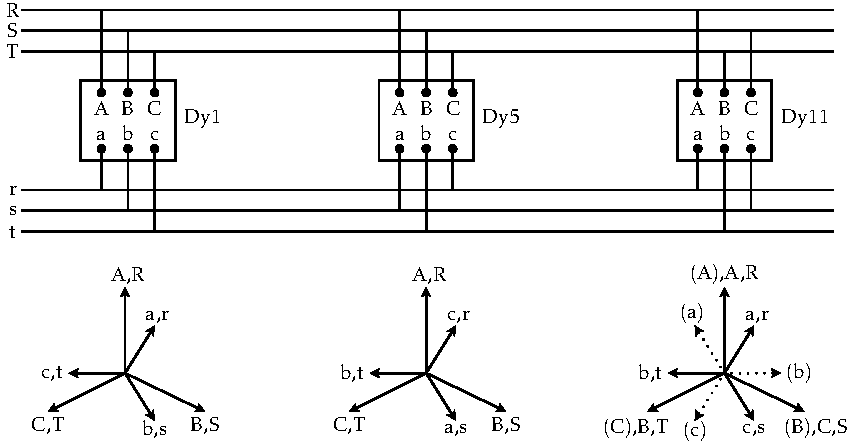
\includegraphics{Imatges/Cap-TrafosPot-Exemple-TR-parallel.pdf}
    \end{figure}

    Comencem connectant el  transformador Dy1 de manera natural, \'{e}s a dir, els debanats primaris A, B i C amb les fases R, S i T respectivament, i els debanats secundaris a, b i c amb les fases r, s i t respectivament.

    Si comparem ara el diagrama de fasors dels transformadors Dy1 i Dy5, veiem que les tensions secund\`{a}ries del Dy5 s\'{o}n les mateixes que les del Dy1 girades $120\degree$. Per tant nom\'{e}s ens cal connectar els debanats primaris com en el cas anterior, i connectar el debanat secundaris c, a i b amb les fases r, s i t respectivament.

    Ens ocupem finalment del transformador Dy11. Si connect\'{e}ssim els debanats primaris com en els dos casos anteriors, tindr\'{\i}em el diagrama de fasors donat per les lletres entre par\`{e}ntesis i les l\'{\i}nies a tra\c{c}os; comparant-lo amb el diagrama de fasors del transformador Dy1, es veu que els fasors (a), (b) i (c) del Dy11 s\'{o}n sim\`{e}trics respecte d'un eix vertical, amb els fasors a, b i c respectivament del Dy1. Per tant si connectem el primari del Dy11 seguint una seq\"{u}\`{e}ncia de tensions inversa, \'{e}s a dir connectem els debanats A, C i B amb les fases R, S i T respectivament, obtindrem un transformador Dy1, com es veu en el diagrama de fasors donat per les lletres sense par\`{e}ntesis i les l\'{\i}nies cont\'{\i}nues; nom\'{e}s cal ara connectar els debanats secundaris a, c i b amb les fases r, s i t respectivament.
\end{exemple}

\subsection{Condicions per a una connexi\'{o} correcta}\index{transformadors de pot\`{e}ncia!connexi\'{o} en para{\l.l}el!connexi\'{o} correcta}
 Es diu que dos transformadors en para{\l.l}el  A i B tenen una connexi\'{o} correcta, quan a m\'{e}s de complir les condicions m\'{\i}nimes de connexi\'{o}, tenen unes tensions de curt circuit iguals:
\begin{align}
    m\ped{A} &= m\ped{B}\\
    h\ped{A} &= h\ped{B}\\
    u\ped{cc,A} &= u\ped{cc,B} \quad (U\ped{cc,A} = U\ped{cc,B})
\end{align}

La condici\'{o} addicional  $u\ped{cc,A} = u\ped{cc,B}$ garanteix que no hi hagi sobrec\`{a}rregues en cap dels transformadors, ja que les intensitats i pot\`{e}ncies es reparteixen entre els dos transformadors de manera proporcional a les seves intensitats nominals; en el cas que les tensions nominals d'A i B siguin a m\'{e}s iguals, es produeix un repartiment proporcional a les seves pot\`{e}ncies nominals.

Per tal que es compleixi $u\ped{cc,A} = u\ped{cc,B}$, la relaci\'{o} entre els valors de placa de caracter\'{\i}stiques $\varepsilon\ped{cc,A}$ i $\varepsilon\ped{cc,B}$ ha de ser:
\begin{equation}
    \varepsilon\ped{cc,B} = \varepsilon\ped{cc,A} \frac{U\ped{N,A}}{U\ped{N,B}}
\end{equation}

\subsection{Condicions per a una connexi\'{o} \`{o}ptima}\index{transformadors de pot\`{e}ncia!connexi\'{o} en para{\l.l}el!connexi\'{o} \`{o}ptima}

 Es diu que dos transformadors en para{\l.l}el A i B tenen una connexi\'{o} \`{o}ptima, quan a m\'{e}s de complir les condicions d'una connexi\'{o} correcta, tenen unes tensions de curt circuit iguals no nom\'{e}s en m\`{o}dul si no tamb\'{e} en argument:
\begin{align}
    m\ped{A} &= m\ped{B}\\
    h\ped{A} &= h\ped{B}\\
    u\ped{cc,A} &= u\ped{cc,B} \quad (U\ped{cc,A} = U\ped{cc,B})\\
    \varphi\ped{cc,A} &=\varphi\ped{cc,B}
\end{align}

La condici\'{o} addicional $\varphi\ped{cc,A} =\varphi\ped{cc,B}$ evita p\`{e}rdues innecess\`{a}ries en el coure, que es produirien en cas contrari.

Per tal que es compleixi $u\ped{cc,A} = u\ped{cc,B} $ i $\varphi\ped{cc,A} =\varphi\ped{cc,B}$, la relaci\'{o} entre els valors de placa de caracter\'{\i}stiques $\varepsilon\ped{cc,A}$, $\varepsilon\ped{cc,B}$, $W\ped{cc,A}$ i $W\ped{cc,B}$ ha de ser:
\begin{equation}
    \varepsilon\ped{cc,B} = \varepsilon\ped{cc,A} \frac{U\ped{N,A}}{U\ped{N,B}} \qquad\qquad
    W\ped{cc,B} = W\ped{cc,A} \frac{S\ped{N,B} \,\varepsilon\ped{cc,B}}{S\ped{N,A}\, \varepsilon\ped{cc,A}}
\end{equation}

\section{Corrent d'irrupci\'{o} ({"<}inrush current{">})}\index{transformadors de pot\`{e}ncia!corrent d'irrupci\'{o} (\guillemotleft inrush current\guillemotright)}\index{corrent d'irrupci\'{o}}\index{inrush current@\guillemotleft inrush current\guillemotright}

El corrent d'irrupci\'{o} s'origina quan es  connecta un transformador a la l\'{\i}nia de pot\`{e}ncia. Aquest corrent \'{e}s de molt curta durada per\`{o} d'un valor molt elevat; el valor dep\`{e}n de l'instant de connexi\'{o} (fase de la tensi\'{o}) i del flux residual del transformador, degut a d'una connexi\'{o} pr\`{e}via.

El corrent d'irrupci\'{o} que circula pel primari pot arribar a valors de fins a $(25\div 30) I\ped{N}$ els primers 10\unit{ms}, corrent que decreix a valors de fins  a $(12\div 15) I\ped{N}$ als 100\unit{ms}.

\section{Designaci\'{o} de les classes de refrigeraci\'{o}}\index{CEI!60076-2}
\index{ANSI!C57.12} \index{transformadors de pot\`{e}ncia!designaci\'{o} de classes de refrigeraci\'{o}}

Les classes de refrigeraci\'{o} utilitzades en els transformadors de
pot\`{e}ncia, es designen mitjan\c{c}ant quatre lletres.

Actualment, la definici\'{o} i l'\'{u}s d'aquestes lletres, \'{e}s coincident
entre la norma europea (\textsf{CEI 60076-2}) i la norma americana
(\textsf{ANSI C57.12}).

Es defineix a continuaci\'{o} el significat d'aquestes lletres:

\textbf{1a lletra}. Indica l'element refrigerant intern, que est\`{a} en
contacte amb els debanats del transformador. Els valors possibles
s\'{o}n els seg\"{u}ents:
\begin{list}{}
   {\setlength{\labelwidth}{10mm} \setlength{\leftmargin}{10mm} \setlength{\labelsep}{2mm}}
   \item[\textbf{O}] L'element refrigerant \'{e}s un oli mineral o un l\'{\i}quid sint\`{e}tic a\"{\i}llant, amb una temperatura d'ignici\'{o}
   inferior o igual a 300\unit{\celsius}.
   \item[\textbf{K}] L'element refrigerant \'{e}s un l\'{\i}quid sint\`{e}tic a\"{\i}llant, amb una temperatura d'ignici\'{o}
   superior a 300\unit{\celsius}.
   \item[\textbf{L}] L'element refrigerant \'{e}s un l\'{\i}quid sint\`{e}tic a\"{\i}llant, amb una temperatura d'ignici\'{o}
   no mesurable.
\end{list}
\index{O} \index{K} \index{L}

\textbf{2a lletra}. Indica el mecanisme de circulaci\'{o} de l'element
refrigerant intern. Els valors possibles s\'{o}n els seg\"{u}ents:
\begin{list}{}
   {\setlength{\labelwidth}{10mm} \setlength{\leftmargin}{10mm} \setlength{\labelsep}{2mm}}
   \item[\textbf{N}] Circulaci\'{o} mitjan\c{c}ant convecci\'{o} natural,
    a trav\'{e}s de l'equip refrigerant i pels debanats del transformador.
   \item[\textbf{F}] Circulaci\'{o} for\c{c}ada a trav\'{e}s de l'equip refrigerant (mitjan\c{c}ant bombes),
    i circulaci\'{o} mitjan\c{c}ant convecci\'{o} natural pels debanats del
    transformador. Aquest tipus de circulaci\'{o} tamb\'{e} s'anomena {"<}de flux no
    dirigit{">}.
   \item[\textbf{D}] Circulaci\'{o} for\c{c}ada a trav\'{e}s de l'equip refrigerant (mitjan\c{c}ant bombes),
    i dirigida per aquest equip refrigerant cap als debanats del
    transformador i, de manera opcional, tamb\'{e} cap a altres parts del transformador. Aquest
    tipus de circulaci\'{o} tamb\'{e} s'anomena {"<}de flux dirigit{">}.
\end{list}
\index{N} \index{F} \index{D}

\textbf{3a lletra}. Indica l'element refrigerant extern. Els valors
possibles s\'{o}n els seg\"{u}ents:
\begin{list}{}
   {\setlength{\labelwidth}{10mm} \setlength{\leftmargin}{10mm} \setlength{\labelsep}{2mm}}
   \item[\textbf{A}] L'element refrigerant \'{e}s l'aire.
   \item[\textbf{W}] L'element refrigerant \'{e}s l'aigua.
\end{list}
\index{A} \index{W}

\textbf{4a lletra}. Indica el mecanisme de circulaci\'{o} de l'element
refrigerant extern. Els valors possibles s\'{o}n els seg\"{u}ents:
\begin{list}{}
   {\setlength{\labelwidth}{10mm} \setlength{\leftmargin}{10mm} \setlength{\labelsep}{2mm}}
   \item[\textbf{N}] Circulaci\'{o} mitjan\c{c}ant convecci\'{o} natural.
   \item[\textbf{F}] Circulaci\'{o} for\c{c}ada, mitjan\c{c}ant ventiladors (en el cas de
   l'aire) o bombes (en el cas de l'aigua).
\end{list}
\index{N} \index{F}

En la Taula \vref{taula:classes-refrigeracio-trafos} es presenta una
comparativa, entres diverses designacions antigues de classes de
refrigeraci\'{o} (segons les normes americanes) i les designacions
equivalents actuals:
\begin{table}[htb]
   \caption{\label{taula:classes-refrigeracio-trafos}
   Classes de refrigeraci\'{o} en els transformadors de pot\`{e}ncia}
   \begin{center}\begin{tabular}{cc}
   \toprule[1pt]
   Designaci\'{o} antiga & Designaci\'{o} actual \\
   (normes \textsf{\textsf{ANSI}})     & (normes \textsf{\textsf{CEI}} i
   \textsf{\textsf{ANSI}}) \\
   \midrule
   OA & ONAN   \\
   FA & ONAF   \\
   FOA & OFAF  \\
   FOW & OFWF  \\
   FOA & ODAF  \\
   FOW & ODWF \\
   \bottomrule[1pt]
   \end{tabular} \end{center}
\end{table}
\index{OA}\index{FA}\index{FOA}\index{FOW}\index{ONAN}\index{ONAF}\index{OFAF}\index{OFWF}\index{ODAF}\index{ODWF}

En el cas d'un transformador on puguem seleccionar que la circulaci\'{o}
sigui natural o for\c{c}ada,
les designacions s\'{o}n del tipus: ONAN/ONAF, ONAN/OFAF, etc.

En el cas dels transformadors secs, l'element refrigerant sempre \'{e}s
l'aire, ja sigui en circulaci\'{o} natural o for\c{c}ada, i per tant les
designacions s\'{o}n simplement AN o AF. 